\documentclass[11pt]{article}
\usepackage{mathblatt}
% gesetzt von werkzeuge/setzer.py aus dem Lernweg (L2-A · L2-B · L2-C · L2-D · L2-T) und den Bankzeilen; Muster T6B.
\input{praeambel}
\newcommand{\kennung}{A5D}
\newcommand{\grau}[1]{{\color{mbgrau}#1}}

\begin{document}
\pfheftstil
\fancyfoot[C]{\parbox[t]{\textwidth}{\mbfhbox\par\vspace{1.5mm}{\footnotesize\color{mbgrau}{\scriptsize \kennung}\hfill\thepage}}}
\pfheftkopf{Kürzen und Erweitern}{Klasse 6}
% L2-A: Erweitern und kürzen
\begin{pfaufg}{}{1.}{}
\gzwei{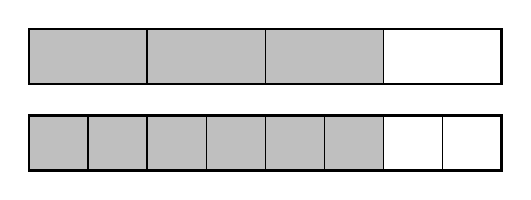
\begin{tikzpicture}[line cap=round]\fill[black!25] (0.000,0.00) rectangle (0.750,0.70);\fill[black!25] (0.750,0.00) rectangle (1.500,0.70);\draw[line width=0.4pt] (0.750,0.00) -- (0.750,0.70);\fill[black!25] (1.500,0.00) rectangle (2.250,0.70);\draw[line width=0.4pt] (1.500,0.00) -- (1.500,0.70);\fill[black!25] (2.250,0.00) rectangle (3.000,0.70);\draw[line width=0.4pt] (2.250,0.00) -- (2.250,0.70);\fill[black!25] (3.000,0.00) rectangle (3.750,0.70);\draw[line width=0.4pt] (3.000,0.00) -- (3.000,0.70);\fill[black!25] (3.750,0.00) rectangle (4.500,0.70);\draw[line width=0.4pt] (3.750,0.00) -- (3.750,0.70);\draw[line width=0.4pt] (4.500,0.00) -- (4.500,0.70);\draw[line width=0.4pt] (5.250,0.00) -- (5.250,0.70);\draw[line width=0.9pt] (0,0.00) rectangle (6.0,0.70);\fill[black!25] (0.000,1.10) rectangle (1.500,1.80);\fill[black!25] (1.500,1.10) rectangle (3.000,1.80);\draw[line width=0.4pt] (1.500,1.10) -- (1.500,1.80);\fill[black!25] (3.000,1.10) rectangle (4.500,1.80);\draw[line width=0.4pt] (3.000,1.10) -- (3.000,1.80);\draw[line width=0.4pt] (4.500,1.10) -- (4.500,1.80);\draw[line width=0.9pt] (0,1.10) rectangle (6.0,1.80);\end{tikzpicture}}{\grau{a)\ Beide Streifen sind gleich lang. Der obere zeigt $\frac{3}{4}$. Der untere ist in 8 gleiche Teile geteilt. Wie viele Teile musst du unten färben, damit gleich viel grau ist?\par\smallskip Jedes Viertel ist unten in 2 Teile geteilt: Aus 4 Teilen werden $4 \cdot 2 = 8$.\par Aus 3 grauen Teilen werden $3 \cdot 2 = 6$. Färbe 6 Teile.\par $\dfrac{3}{4} = \dfrac{3 \cdot 2}{4 \cdot 2} = \dfrac{6}{8}$. Das heißt: mit 2 \textbf{erweitert}.\par Von unten nach oben gelesen: $\dfrac{6}{8} = \dfrac{6 : 2}{8 : 2} = \dfrac{3}{4}$. Das heißt: mit 2 \textbf{gekürzt}.}}
\par\medskip
\gzwei{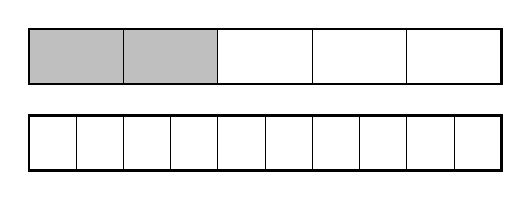
\begin{tikzpicture}[line cap=round]\draw[line width=0.4pt] (0.600,0.00) -- (0.600,0.70);\draw[line width=0.4pt] (1.200,0.00) -- (1.200,0.70);\draw[line width=0.4pt] (1.800,0.00) -- (1.800,0.70);\draw[line width=0.4pt] (2.400,0.00) -- (2.400,0.70);\draw[line width=0.4pt] (3.000,0.00) -- (3.000,0.70);\draw[line width=0.4pt] (3.600,0.00) -- (3.600,0.70);\draw[line width=0.4pt] (4.200,0.00) -- (4.200,0.70);\draw[line width=0.4pt] (4.800,0.00) -- (4.800,0.70);\draw[line width=0.4pt] (5.400,0.00) -- (5.400,0.70);\draw[line width=0.9pt] (0,0.00) rectangle (6.0,0.70);\fill[black!25] (0.000,1.10) rectangle (1.200,1.80);\fill[black!25] (1.200,1.10) rectangle (2.400,1.80);\draw[line width=0.4pt] (1.200,1.10) -- (1.200,1.80);\draw[line width=0.4pt] (2.400,1.10) -- (2.400,1.80);\draw[line width=0.4pt] (3.600,1.10) -- (3.600,1.80);\draw[line width=0.4pt] (4.800,1.10) -- (4.800,1.80);\draw[line width=0.9pt] (0,1.10) rectangle (6.0,1.80);\end{tikzpicture}}{%
b)\ Beide Streifen sind gleich lang. Der obere zeigt $\frac{2}{5}$. Färbe im unteren Streifen gleich viel. Welcher Bruch steht dann unten?\karo{3}}
\fusshilfe{\mbox{1:~b) $\frac{4}{10}$ (4 Teile färben)}}
\end{pfaufg}

% L2-A: Erweitern und kürzen
\begin{pfaufg}{}{2.}{}
Erweitert oder gekürzt – und mit welcher Zahl? \par\vspace{3pt} a)~$\dfrac{4}{9} = \dfrac{20}{45}$ \qquad b)~$\dfrac{21}{28} = \dfrac{3}{4}$ \qquad c)~$\dfrac{5}{8} = \dfrac{40}{64}$\karo{3}
\fusshilfe{\mbox{2:~a) mal 5 \quad b) durch 7 \quad c) mal 8}}
\end{pfaufg}

% L2-A: Erweitern und kürzen
\begin{pfaufg}{}{3.}{}
Erweitere mit der Zahl in Klammern. \par\vspace{3pt} a)~$\dfrac{3}{5}$ (mit 4) \qquad b)~$\dfrac{5}{6}$ (mit 3) \qquad c)~$\dfrac{7}{9}$ (mit 10)\karo{3}
\fusshilfe{\mbox{3:~a) $\frac{12}{20}$ \quad b) $\frac{15}{18}$ \quad c) $\frac{70}{90}$}}
\end{pfaufg}

% L2-A: Erweitern und kürzen
\begin{pfaufg}{}{4.}{}
Kürze mit der Zahl in Klammern. \par\vspace{3pt} a)~$\dfrac{20}{24}$ (mit 4) \qquad b)~$\dfrac{15}{35}$ (mit 5) \qquad c)~$\dfrac{24}{42}$ (mit 6)\karo{3}
\fusshilfe{\mbox{4:~a) $\frac{5}{6}$ \quad b) $\frac{3}{7}$ \quad c) $\frac{4}{7}$}}
\end{pfaufg}

% L2-A: Erweitern und kürzen
\begin{pfaufg}{}{5.}{}
Lena bricht ihren Schokoriegel in 4 gleiche Stücke und isst 3 davon. Tom bricht einen gleich großen Riegel in 12 gleiche Stücke und isst 9 davon. Wer hat mehr gegessen?\karo{3}
\fusshilfe{\mbox{5:~gleich viel}}
\end{pfaufg}

% L2-B: Vollständig kürzen
\begin{pfaufg}{}{6.}{}
\grau{a)\ Kürze $\frac{30}{42}$ vollständig.\par\smallskip Beide Zahlen sind gerade: durch 2. \ $\dfrac{30}{42} = \dfrac{15}{21}$\par 15 und 21 stehen beide in der Dreierreihe: durch 3. \ $\dfrac{15}{21} = \dfrac{5}{7}$\par 5 und 7 teilt keine Zahl außer 1. Fertig: $\dfrac{30}{42} = \dfrac{5}{7}$\par Schneller geht es mit einem Schritt: durch 6, die größte Zahl, die 30 und 42 teilt.}
\par\medskip
b)\ Kürze vollständig. \par\vspace{3pt} a)~$\dfrac{6}{8}$ \qquad b)~$\dfrac{10}{15}$ \qquad c)~$\dfrac{8}{20}$\karo{3}
\fusshilfe{\mbox{6:~b) a) $\frac{3}{4}$ \quad b) $\frac{2}{3}$ \quad c) $\frac{2}{5}$}}
\end{pfaufg}

% L2-B: Vollständig kürzen
\begin{pfaufg}{}{7.}{}
Kürze vollständig. Prüfe nach jedem Kürzen, ob es noch weiter geht. \par\vspace{3pt} a)~$\dfrac{18}{24}$ \qquad b)~$\dfrac{36}{60}$ \qquad c)~$\dfrac{48}{72}$\karo{3}
\fusshilfe{\mbox{7:~a) $\frac{3}{4}$ \quad b) $\frac{3}{5}$ \quad c) $\frac{2}{3}$}}
\end{pfaufg}

% L2-B: Vollständig kürzen
\begin{pfaufg}{}{8.}{}
\gzwei{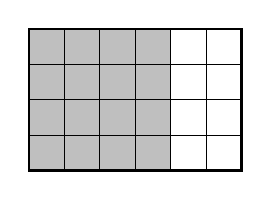
\begin{tikzpicture}[line cap=round]\fill[black!25] (0.00,1.35) rectangle (0.45,1.80);\fill[black!25] (0.45,1.35) rectangle (0.90,1.80);\fill[black!25] (0.90,1.35) rectangle (1.35,1.80);\fill[black!25] (1.35,1.35) rectangle (1.80,1.80);\fill[black!25] (0.00,0.90) rectangle (0.45,1.35);\fill[black!25] (0.45,0.90) rectangle (0.90,1.35);\fill[black!25] (0.90,0.90) rectangle (1.35,1.35);\fill[black!25] (1.35,0.90) rectangle (1.80,1.35);\fill[black!25] (0.00,0.45) rectangle (0.45,0.90);\fill[black!25] (0.45,0.45) rectangle (0.90,0.90);\fill[black!25] (0.90,0.45) rectangle (1.35,0.90);\fill[black!25] (1.35,0.45) rectangle (1.80,0.90);\fill[black!25] (0.00,0.00) rectangle (0.45,0.45);\fill[black!25] (0.45,0.00) rectangle (0.90,0.45);\fill[black!25] (0.90,0.00) rectangle (1.35,0.45);\fill[black!25] (1.35,0.00) rectangle (1.80,0.45);\draw[line width=0.4pt] (0,0) grid[step=0.45] (2.70,1.80);\draw[line width=0.9pt] (0,0) rectangle (2.70,1.80);\end{tikzpicture}}{%
Die Figur besteht aus gleich großen Kästchen. Welcher Anteil der Figur ist grau? Gib ihn vollständig gekürzt an.\karo{3}}
\fusshilfe{\mbox{8:~$\frac{16}{24} = \frac{2}{3}$}}
\end{pfaufg}

% L2-B: Vollständig kürzen
\begin{pfaufg}{}{9.}{}
Welcher Bruchteil des Ganzen ist das? Gib ihn vollständig gekürzt an. \par a)~50 min von 1 h \qquad b)~750 g von 1 kg \qquad c)~35 cm von 1 m\karo{3}
\fusshilfe{\mbox{9:~a) $\frac{5}{6}$ \quad b) $\frac{3}{4}$ \quad c) $\frac{7}{20}$}}
\end{pfaufg}

% L2-B: Vollständig kürzen
\begin{pfaufg}{}{10.}{}
Tim hat im Test 21 von 28 Punkten. Er sagt: „Das sind drei Viertel der Punkte.“ Hat er recht?\karo{3}
\fusshilfe{\mbox{10:~Ja}}
\end{pfaufg}

% L2-C: Auf einen gemeinsamen Nenner bringen
\begin{pfaufg}{}{11.}{}
\grau{a)\ Mache $\frac{3}{4}$ und $\frac{5}{6}$ gleichnamig.\par\smallskip Gemeinsamen Nenner suchen. Sechserreihe: 6, 12 – und 12 steht auch in der Viererreihe.\par Mit welcher Zahl erweitern? \ $12 : 4 = 3$ \ und \ $12 : 6 = 2$\par $\dfrac{3}{4} = \dfrac{3 \cdot 3}{4 \cdot 3} = \dfrac{9}{12}$ \ und \ $\dfrac{5}{6} = \dfrac{5 \cdot 2}{6 \cdot 2} = \dfrac{10}{12}$}
\par\medskip
b)\ Schreibe mit dem Nenner 24. \par\vspace{3pt} a)~$\dfrac{2}{3}$ \qquad b)~$\dfrac{5}{8}$ \qquad c)~$\dfrac{7}{12}$\karo{3}
\fusshilfe{\mbox{11:~b) a) $\frac{16}{24}$ \quad b) $\frac{15}{24}$ \quad c) $\frac{14}{24}$}}
\end{pfaufg}

% L2-C: Auf einen gemeinsamen Nenner bringen
\begin{pfaufg}{}{12.}{}
Schreibe mit dem Nenner 100 und gib den Anteil in Prozent an ($\frac{1}{100} = 1\,\%$). \par\vspace{3pt} a)~$\dfrac{3}{10}$ \qquad b)~$\dfrac{7}{20}$ \qquad c)~$\dfrac{12}{25}$\karo{3}
\fusshilfe{\mbox{12:~a) $30\,\%$ \quad b) $35\,\%$ \quad c) $48\,\%$}}
\end{pfaufg}

% L2-C: Auf einen gemeinsamen Nenner bringen
\begin{pfaufg}{}{13.}{}
Mache gleichnamig. Ein Nenner steckt schon im anderen. \par\vspace{3pt} a)~$\dfrac{2}{3}$ und $\dfrac{7}{9}$ \qquad b)~$\dfrac{1}{4}$ und $\dfrac{5}{12}$ \qquad c)~$\dfrac{3}{5}$ und $\dfrac{11}{20}$\karo{3}
\fusshilfe{\mbox{13:~a) $\frac{6}{9}$ \quad b) $\frac{3}{12}$ \quad c) $\frac{12}{20}$}}
\end{pfaufg}

% L2-C: Auf einen gemeinsamen Nenner bringen
\begin{pfaufg}{}{14.}{}
Mache gleichnamig. \par\vspace{3pt} a)~$\dfrac{1}{6}$ und $\dfrac{3}{4}$ \qquad b)~$\dfrac{2}{5}$ und $\dfrac{1}{3}$ \qquad c)~$\dfrac{5}{8}$ und $\dfrac{7}{12}$\karo{3}
\fusshilfe{\mbox{14:~Nenner 12; 15; 24}}
\end{pfaufg}

% L2-C: Auf einen gemeinsamen Nenner bringen
\begin{pfaufg}{}{15.}{}
Jonas hat beim Training 21 von 25 Elfmetern verwandelt, Mia 17 von 20. Wer trifft besser? Vergleiche die Anteile in Prozent.\karo{3}
\fusshilfe{\mbox{15:~Mia}}
\end{pfaufg}

% L2-D: Brüche größer als 1: gemischte Zahlen
\begin{pfaufg}{}{16.}{}
\gzwei{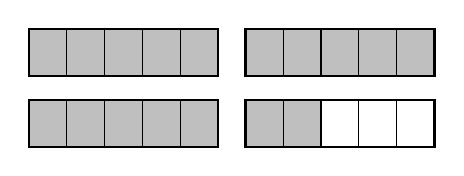
\begin{tikzpicture}[line cap=round]\fill[black!25] (0.000,0.00) rectangle (0.480,0.60);\fill[black!25] (0.480,0.00) rectangle (0.960,0.60);\draw[line width=0.4pt] (0.480,0.00) -- (0.480,0.60);\fill[black!25] (0.960,0.00) rectangle (1.440,0.60);\draw[line width=0.4pt] (0.960,0.00) -- (0.960,0.60);\fill[black!25] (1.440,0.00) rectangle (1.920,0.60);\draw[line width=0.4pt] (1.440,0.00) -- (1.440,0.60);\fill[black!25] (1.920,0.00) rectangle (2.400,0.60);\draw[line width=0.4pt] (1.920,0.00) -- (1.920,0.60);\draw[line width=0.9pt] (0.000,0.00) rectangle (2.400,0.60);\fill[black!25] (2.750,0.00) rectangle (3.230,0.60);\fill[black!25] (3.230,0.00) rectangle (3.710,0.60);\draw[line width=0.4pt] (3.230,0.00) -- (3.230,0.60);\fill[black!25] (3.710,0.00) rectangle (4.190,0.60);\draw[line width=0.4pt] (3.710,0.00) -- (3.710,0.60);\fill[black!25] (4.190,0.00) rectangle (4.670,0.60);\draw[line width=0.4pt] (4.190,0.00) -- (4.190,0.60);\fill[black!25] (4.670,0.00) rectangle (5.150,0.60);\draw[line width=0.4pt] (4.670,0.00) -- (4.670,0.60);\draw[line width=0.9pt] (2.750,0.00) rectangle (5.150,0.60);\fill[black!25] (0.000,-0.90) rectangle (0.480,-0.30);\fill[black!25] (0.480,-0.90) rectangle (0.960,-0.30);\draw[line width=0.4pt] (0.480,-0.90) -- (0.480,-0.30);\fill[black!25] (0.960,-0.90) rectangle (1.440,-0.30);\draw[line width=0.4pt] (0.960,-0.90) -- (0.960,-0.30);\fill[black!25] (1.440,-0.90) rectangle (1.920,-0.30);\draw[line width=0.4pt] (1.440,-0.90) -- (1.440,-0.30);\fill[black!25] (1.920,-0.90) rectangle (2.400,-0.30);\draw[line width=0.4pt] (1.920,-0.90) -- (1.920,-0.30);\draw[line width=0.9pt] (0.000,-0.90) rectangle (2.400,-0.30);\fill[black!25] (2.750,-0.90) rectangle (3.230,-0.30);\fill[black!25] (3.230,-0.90) rectangle (3.710,-0.30);\draw[line width=0.4pt] (3.230,-0.90) -- (3.230,-0.30);\draw[line width=0.4pt] (3.710,-0.90) -- (3.710,-0.30);\draw[line width=0.4pt] (4.190,-0.90) -- (4.190,-0.30);\draw[line width=0.4pt] (4.670,-0.90) -- (4.670,-0.30);\draw[line width=0.9pt] (2.750,-0.90) rectangle (5.150,-0.30);\end{tikzpicture}}{\grau{a)\ Schreibe $\frac{17}{5}$ als gemischte Zahl.\par\smallskip Wie viele Ganze? \ $17 : 5 = 3$ Rest $2$\par 3 ganze Streifen und 2 Fünftel: \ $\dfrac{17}{5} = 3\dfrac{2}{5}$\par Probe rückwärts: $3 \cdot 5 + 2 = 17$, also $3\dfrac{2}{5} = \dfrac{17}{5}$.}}
\par\medskip
b)\ Schreibe als gemischte Zahl. \par\vspace{3pt} a)~$\dfrac{7}{2}$ \qquad b)~$\dfrac{11}{3}$ \qquad c)~$\dfrac{23}{4}$\karo{3}
\fusshilfe{\mbox{16:~b) a) $3\frac{1}{2}$ \quad b) $3\frac{2}{3}$ \quad c) $5\frac{3}{4}$}}
\end{pfaufg}

% L2-D: Brüche größer als 1: gemischte Zahlen
\begin{pfaufg}{}{17.}{}
Schreibe als Bruch. \par\vspace{3pt} a)~$1\dfrac{3}{4}$ \qquad b)~$2\dfrac{5}{6}$ \qquad c)~$4\dfrac{2}{9}$\karo{3}
\fusshilfe{\mbox{17:~a) $\frac{7}{4}$ \quad b) $\frac{17}{6}$ \quad c) $\frac{38}{9}$}}
\end{pfaufg}

% L2-D: Brüche größer als 1: gemischte Zahlen
\begin{pfaufg}{}{18.}{}
Schreibe als Bruch. Ist er größer als 1, schreibe ihn auch als gemischte Zahl. \par a)~$5 : 8$ \qquad b)~$9 : 4$ \qquad c)~$20 : 6$\karo{3}
\fusshilfe{\mbox{18:~a) $\frac{5}{8}$ \quad b) $2\frac{1}{4}$ \quad c) $3\frac{1}{3}$}}
\end{pfaufg}

% L2-D: Brüche größer als 1: gemischte Zahlen
\begin{pfaufg}{}{19.}{}
Ein Film dauert 135 Minuten. Wie viele Stunden sind das? Schreibe als gemischte Zahl.\karo{3}
\fusshilfe{\mbox{19:~$2\frac{1}{4}$\,h}}
\end{pfaufg}

% L2-D: Brüche größer als 1: gemischte Zahlen
\begin{pfaufg}{}{20.}{}
Für das Klassenfrühstück werden 14 Baguettes gerecht auf 4 Tische verteilt. Wie viele Baguettes bekommt jeder Tisch? Wie schneidet man die übrigen?\karo{3}
\fusshilfe{\mbox{20:~$3\frac{1}{2}$ je Tisch}}
\end{pfaufg}

% L2-T: Probetest
\begin{pfaufg}{}{21.}{}
Ergänze die fehlende Zahl. \par\vspace{3pt} a)~$\dfrac{3}{8} = \dfrac{\square}{40}$ \qquad b)~$\dfrac{28}{35} = \dfrac{4}{\square}$ \qquad c)~$\dfrac{5}{\square} = \dfrac{30}{42}$\karo{3}
\fusshilfe{\mbox{21:~a) 15 \quad b) 5 \quad c) 7}}
\end{pfaufg}

% L2-T: Probetest
\begin{pfaufg}{}{22.}{}
Kürze vollständig. \par\vspace{3pt} a)~$\dfrac{24}{32}$ \qquad b)~$\dfrac{45}{75}$ \qquad c)~$\dfrac{36}{54}$\karo{3}
\fusshilfe{\mbox{22:~a) $\frac{3}{4}$ \quad b) $\frac{3}{5}$ \quad c) $\frac{2}{3}$}}
\end{pfaufg}

% L2-T: Probetest
\begin{pfaufg}{}{23.}{}
Mache gleichnamig. \par\vspace{3pt} a)~$\dfrac{5}{6}$ und $\dfrac{4}{9}$ \qquad b)~$\dfrac{3}{10}$ und $\dfrac{1}{4}$\karo{3}
\fusshilfe{\mbox{23:~Nenner 18; 20}}
\end{pfaufg}

% L2-T: Probetest
\begin{pfaufg}{}{24.}{}
Schreibe um. \par\vspace{3pt} a)~$\dfrac{29}{6}$ als gemischte Zahl \qquad b)~$3\dfrac{3}{8}$ als Bruch \qquad c)~$13 : 5$ als gemischte Zahl\karo{3}
\fusshilfe{\mbox{24:~a) $4\frac{5}{6}$ \quad b) $\frac{27}{8}$ \quad c) $2\frac{3}{5}$}}
\end{pfaufg}

% L2-T: Probetest
\begin{pfaufg}{}{25.}{}
\gzwei{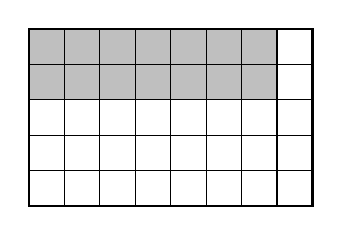
\begin{tikzpicture}[line cap=round]\fill[black!25] (0.00,1.80) rectangle (0.45,2.25);\fill[black!25] (0.45,1.80) rectangle (0.90,2.25);\fill[black!25] (0.90,1.80) rectangle (1.35,2.25);\fill[black!25] (1.35,1.80) rectangle (1.80,2.25);\fill[black!25] (1.80,1.80) rectangle (2.25,2.25);\fill[black!25] (2.25,1.80) rectangle (2.70,2.25);\fill[black!25] (2.70,1.80) rectangle (3.15,2.25);\fill[black!25] (0.00,1.35) rectangle (0.45,1.80);\fill[black!25] (0.45,1.35) rectangle (0.90,1.80);\fill[black!25] (0.90,1.35) rectangle (1.35,1.80);\fill[black!25] (1.35,1.35) rectangle (1.80,1.80);\fill[black!25] (1.80,1.35) rectangle (2.25,1.80);\fill[black!25] (2.25,1.35) rectangle (2.70,1.80);\fill[black!25] (2.70,1.35) rectangle (3.15,1.80);\draw[line width=0.4pt] (0,0) grid[step=0.45] (3.60,2.25);\draw[line width=0.9pt] (0,0) rectangle (3.60,2.25);\end{tikzpicture}}{%
Die Figur besteht aus gleich großen Kästchen. Welcher Anteil der Fläche ist grau? Gib ihn als vollständig gekürzten Bruch und in Prozent an.\karo{3}}
\fusshilfe{\mbox{25:~$\frac{7}{20} = 35\,\%$}}
\end{pfaufg}

% L2-T: Probetest
\begin{pfaufg}{}{26.}{}
Beim Sportfest gibt es eine Urkunde, wenn man mindestens drei Viertel der möglichen Punkte holt. Ole hat 33 von 44 Punkten, Ida 26 von 36 Punkten. Wer bekommt eine Urkunde?\karo{3}
\fusshilfe{\mbox{26:~nur Ole}}
\end{pfaufg}

\par\vfill\noindent{\footnotesize Vorher: Bruch als Anteil\quad\textbullet\quad Weiter: Brüche vergleichen\par}
\end{document}
